\documentclass[8pt]{article}
\usepackage{geometry}                % See geometry.pdf to learn the layout options. There are lots.
\geometry{letterpaper}                   % ... or a4paper or a5paper or ... 
%\geometry{landscape}                % Activate for for rotated page geometry
%\usepackage[parfill]{parskip}    % Activate to begin paragraphs with an empty line rather than an indent
\usepackage{graphicx}
\usepackage{amssymb}
\usepackage{epstopdf}
\DeclareGraphicsRule{.tif}{png}{.png}{`convert #1 `dirname #1`/`basename #1 .tif`.png}
\graphicspath{{/Users/marlon/Documents/BA/thesis/pictures/}}

\title{Unsupervised Cognate Identification with Variational Autoencoders}
\author{Marlon Betz}
%\date{}                                           % Activate to display a given date or no date

\begin{document}
\maketitle
\newpage
\tableofcontents
\section{Introduction}

Historical Linguistics investigates language from a diachronic perspective, i.e. it seeks to uncover the history of languages and the structure of the hidden forces that drive language change.  Computational Historical Linguistics accordingly deals with computational methods to explore the history of languages and topics closely related to it, such as phylogenetic inferences of language families \cite{bouckaert2012mapping}, migration of language speakers \cite{gray2009language}, inferring lexical flows between languages \cite{dellert2015uralic} or modeling sound change \cite{bouchard2013automated}.  

On the other hand, deep neural networks have been proven to uncover latent features of data and use them for a variety of tasks. However, Computation Historical Linguistics has hardly been touched yet by the current Deep Learning boom (a notable exception is \cite{rama2016siamese}). 
The aim of this thesis is hence 
\begin{enumerate}
\item to propose a model of modeling sound change as a walk in latent space, which is suitable for deep neural networks
\item to use variational autoencoders as a means to uncover the the latent structure that describes the connection between the phonological shape and  the meaning of a given word as well as the geographical location of the speakers of the language the word belongs to, and to investigate it
\item to show how this uncovered structure can be used to identify cognates in an unsupervised way
\end{enumerate}

I will first start by giving an overview of the problem of cognate identification and related fields of research. I will give a background on why cognate identification is important to discuss the historical connections between languages and further provide an overview on several established methods to detect cognates.  

Then I will proceed to introduce the concept of sound change as a walk in latent space, which serves as a background for the actual inference model. Here I will talk about the main motivations for this approach as well as its major drawbacks. 


I will then discuss the actual architecture of the inference model. This first covers a general overview on the components included in the model. I will then in detail look over all components in particular. That will first cover a discussion of different methods of phoneme vectorizations. This is followed by a general overview on autoencoders as non-linear dimensionality reduction architectures first and then a description of variational autoencoders in particular, which build the backbone of the model described here. I then come to the discussion of possible ways to cluster the words, i.e. to assign the actual inferred cognacy labels.

Then I will document how well those methods can be used to infer cognacy between words. I will compare the inferred labels with expert judgements first and then see how the inferred labels can infer language phylogenies, using established bayesian models of cognate evolution.

Finally, I will give a resume on the model described here.

\section{Motivation}

\section{Sound Change as a Walk in Latent Space}
\label{Sound Change as a Walk in Latent Space}
Sound change is usually described as a change of distinctive phonological features.
Accordingly, a sound change such as final devoicing as in 

\begin{equation}
MHG /hund/ \rightarrow NHG /hunt/
\end{equation}

 would be captured by a rule like
\begin{equation}
\textsc{[+voice]} \rightarrow \textsc{[-voice]} / \_ \#
\label{eq:final_devoicing}
\end{equation}
which describes the loss of voice at the end of a word. 


If we use 

If we have established such a latent feature space $\mathbb{R}^n$, a sound change $sc$ that derives a recent form of word $w_{recent}$ from an ancient form  $w_{ancient}$ should then correspond to a vector $v_{sc}$ in such a way that 
\begin{equation}
v_{w_{ancient}}+v_{sc} = v_{w_{recent}}
\end{equation}
From this follows that 

\begin{equation}
v_{sc} =  v_{w_{recent}} - v_{w_{ancient}} 
\end{equation}

That is, we can formulate sound changes such as \ref{eq:final_devoicing} without neither the actual sound change nor the conditioning specifying where the sound change should apply, but only the respective words involved.
If we further assume that that sound change affects another word $w'$, we have

\begin{equation}
v_{w_{recent}} - v_{w_{ancient}}  =  v_{w'_{recent}} - v_{w'_{ancient}} 
\end{equation}
which is equivalent to
\begin{equation}
v_{w_{recent}}  =   v_{w_{ancient}}  + (v_{w'_{recent}} - v_{w'_{ancient}}) 
\end{equation}
If we want to evaluate that latent feature space, we investigate in how far that compositional structure is preserved in our latent space. In fact, such analogy tasks can be used as an evaluation method to test whether the learned embedding space encodes the structure expected to be inherently contained in the data \cite{mikolov2013distributed}.

As we usually do not know the ancient version of a word but only recent ones, we expect the cognates to have spread in the feature space from the origin to some directions.
\begin{equation}
v_{w_{recent}} \sim \mathcal{N}(\mu = v_{w_{ancient}},\sigma ^2 I)
\end{equation}

\section{Related Research}
\section{Architecture}
Hence, the model should have three major components:
\begin{enumerate}
\item The phonemes should be embedded in a feature space, where similar phonemes should cluster in similar subspaces of the feature space. 
\item The words as sequences of such phoneme embeddings should themselves be embedded in another feature space, where words with similar shape should cluster among each other. 
\item The word embeddings are then clustered in such a way that words that appear together in a cluster are assigned a common label, which is then predicted cognate class.
\end{enumerate}

\subsection{Phoneme Vectorization}
\subsubsection{Hand-crafted Vectorization Models}
\subsubsection{Data-driven Embeddings}

\begin{figure}[htbp]
\begin{center}
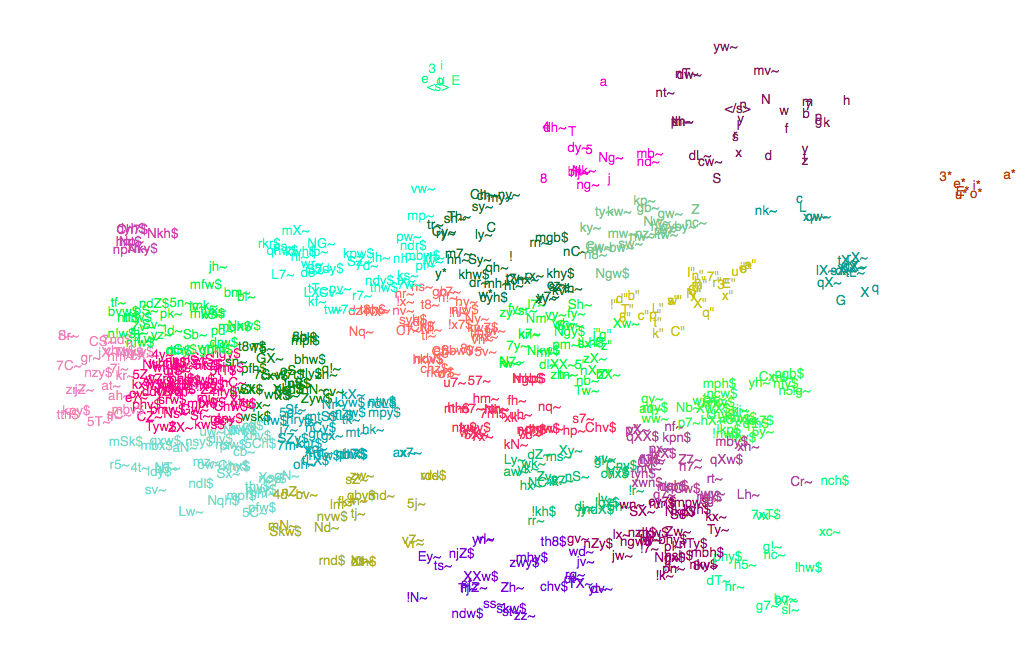
\includegraphics[width=\textwidth]{phoneme_embeddings_overview_ap} 
\caption{T-SNE visualization of the embeddings of all 720 phonemes contained in ASJP, trained with word2vec. The colors represent clusters inferred by Affinity Propagation. The model can clearly separate vowels and various forms of special articulation types. Pulmonic consonants can also be separated clearly from other coarticulation variants, as can uvular or pre-nasalized sounds. Less frequent phonemes, however, cannot be clearly differentiated. }
\label{default}
\end{center}
\end{figure}



If we assume that phonemes do not change unconditionally nor randomly, but instead only change distinctive features given the context the phonemes to change appear in, it should be able to embed phonemes in a latent space where local subspaces contain clusters of phonemes that appear in similar environments. 

That is, we train a model that either predicts the phoneme given its context or vice versa.  
\subsection{Word Embeddings}

\subsubsection{Autoencoders}
\subsubsection{Variational Autoencoders}

Following this, 4 different models are investigated here:
\begin{enumerate}
\item A model that tries to maximize $p(W=w|z;W)$, i.e. that learns the manifold creating the words as such
\item A model that tries to maximize $p(W=w,C=c|z;W,C)$, i.e. that learns the manifold creating the words and the respective concepts
\item A model that tries to maximize $p(W=w,C=c,G=g|z;W,C,G)$, i.e. that learns the manifold creating the words, the respective concepts and the geographical location
\item A model that tries to maximize $p(W=w|z,C=c;W)$, i.e that learns the manifold creating words given the respective concept.
\end{enumerate}

\subsection{Clustering}
\subsubsection{Affinity Propagation}
\section{Evaluation}
\subsection{Data}
\subsection{Results}
\section{Resume}
\section{Acknowledgements}
For training the phoneme embeddings, I used the word2vec implementations provided by the gensim package \cite{rehurek_lrec}. The Autoencoder was implemented with Keras \cite{chollet2015keras} and Tensorflow \cite{tensorflow2015-whitepaper}. The clustering algorithms used here were provided by scikit-learn \cite{scikit-learn}. All code connected to this thesis can be found on my github \footnote{https://github.com/marlonbetz/BA}
%\subsection{}


\bibliographystyle{apa}
\bibliography{references}
\end{document}  